\section{Anexos}

\subsection{Organización del código fuente}
El proyecto completo se encuentra separado en cuatro aplicaciones: Maestro ATmega328P, Slave 1, Slave 2 y ESP32. Los proyectos de los ATmega328P incluyen librerías propias para I2C, protocolo, sensores y actuadores. El Maestro incorpora además LCD, VL53L0X, base de tiempo, UART y la recepción UART por software desde el ESP32.

El código del ESP32 se encuentra en el archivo \texttt{implementacionadafruit.ino} y contiene la integración con \texttt{AdafruitIO\_WiFi}, UART2 y los ocho feeds descritos en este informe.

Por seguridad, las credenciales WiFi y las claves privadas de servicios externos no deben reproducirse en el trabajo escrito ni publicarse en un repositorio abierto. Antes de realizar la entrega en GitHub se recomienda sustituirlas por constantes de ejemplo o almacenarlas en un archivo local excluido mediante \texttt{.gitignore}.

Los archivos completos de código se entregan en el repositorio del proyecto; en el cuerpo del informe se presentan únicamente las estructuras y fragmentos necesarios para explicar la implementación.

\subsection{Video de demostración}
Como evidencia adicional del funcionamiento e integración del prototipo se registró un video de demostración y se publicó en YouTube como parte de los entregables del proyecto.

\begin{figure}[H]
    \centering
    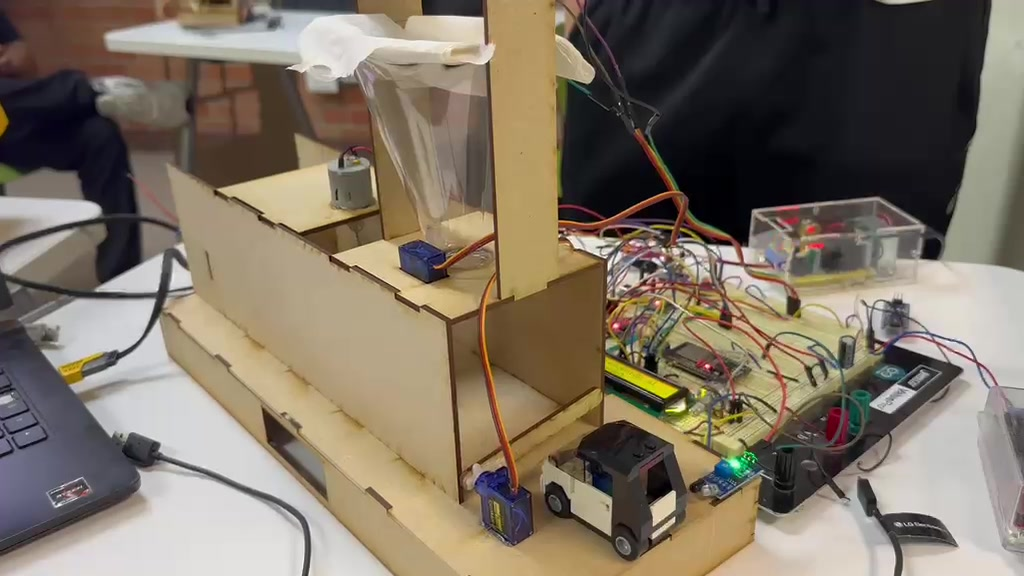
\includegraphics[width=0.78\textwidth]{imagenes/video_demostracion.jpg}
    \caption{Fotograma del video de demostración del prototipo durante las pruebas de funcionamiento.}
\end{figure}

El video de demostración se encuentra disponible en YouTube en el siguiente enlace: \href{https://youtu.be/x-vYncTifNw}{https://youtu.be/x-vYncTifNw}.
